\subsubsection{Scenarios}
\begin{flushleft}\emph{\textbf{Scenario 1}}\end{flushleft}

Lorenzo is a student who is living in Rome. During the summer, he decides to go on a trip to Milan. Due to the fact that Milan is a really crowded city and number of accidents and traffic violations have skyrocketed in the recent decade, he is skeptical to drive his personal car to enjoy the eye-catching scenery along the way or book a flight. His friend suggests to use the SafeStreets app to check the safety of the area he will be staying in Milan in order to decide whether it would be safe to leave his car behind and move on foot there. Therefore he goes on his phone app store and installs the app. Then he fills up all the required fields in the registration form. Then he stays for the verification of his account by SMS and Email. After Lorenzo's account is verified, he goes to login in the app, so he entered his credentials for login and logs into the app so he is redirected to the homepage. He gets a message from the app asking permission to access his mobile phone camera; he accepts. He then gets a second message to give permission to the app to access his current location; he accepts this as well. Then Lorenzo opens the View Safety section and searches for the area around his hotel.

\begin{flushleft}\emph{\textbf{Scenario 2}}\end{flushleft}


Paul is walking on the sidewalk near his home when he notices in the distance a car parked on the sidewalk obstructing his way. He decides to report this since it poses a threat to the safety of people walking by. Paul opens the \emph{SafeStreets} app on his mobile phone to make the report. He takes a photo of the violating vehicle showing the license plate number, The plate number is detected and shown in text on the app. He indicates the type of violation . The location of the violation is detected using Paul's current location. After submitting the report, he gets the feeling that this is not the first time he reports this car for parking of the sidewalk near his house; therefore, he opens the Report History section of the app and searches for his reports from the last month to check if he was right.

\subsubsection{UseCase Diagram}
The following usecase diagram show the different usecases to be described in the following subsections and the relations and interactions among them and with the system users. The users, shown as actors initiate the different usecases some of which initiate other usecases such as the register usecase which initiates the login.

\begin{figure}[H]
\begin{flushleft}\emph{\textbf{Use Case Diagram}}\end{flushleft}
\caption{Use Case Diagram}
\label{usecase}
\centering
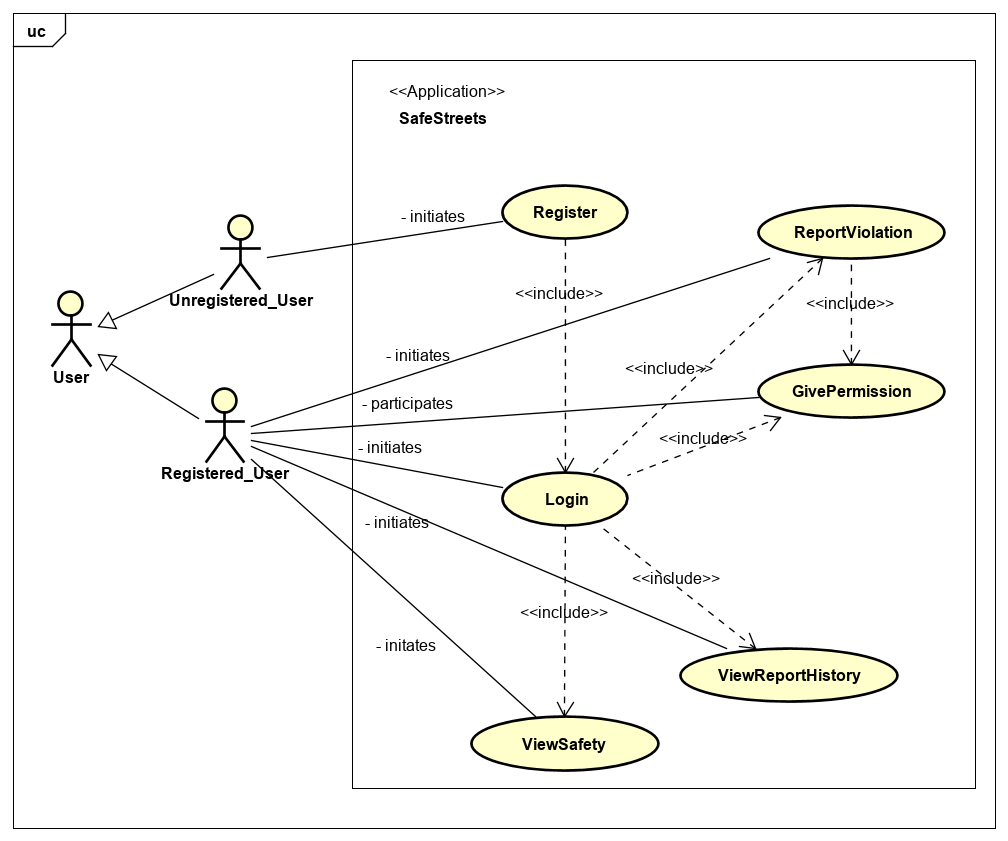
\includegraphics[width=\textwidth, height=0.80\textheight]{usecase-diagram.png}
\end{figure}
\paragraph{Registration}
\hfill \break

\subsubsection{General Functions}

\import{/}{User-General-Functions}

\subsubsection{Violation Report}

\import{/}{User-Violation-Report}

\subsubsection{View Safety}

\import{/}{User-View-Safety}

\subsubsection{Requirements}
In the following section the functional requirements of the system will be discussed. The requirements shall be grouped together by the various main functions of the system that they are related to.


\textbf{General User Functions:}

\begin{itemize}
	\item \requirement{1}
	\item \requirement{2}
	\item \requirement{3}
	\item \requirement{4}
\end{itemize}

	

\textbf{User Violation Reporting:}

\begin{itemize}
	\item \requirement{5}
	\item \requirement{6}
	\item \requirement{7}
	\item \requirement{8}
	\item \requirement{9}
\end{itemize}


\textbf{User View Area Safety:}

\begin{itemize}
\item \requirement{10}
	\item \requirement{11}
	\item \requirement{12}
	\item \requirement{13}
	\item \requirement{14}
	
\end{itemize}

\textbf{User Report History:}

\begin{itemize}
	\item \requirement{15}
\end{itemize}



\textbf{Municipality Interaction:}

\begin{itemize}
\item \requirement{16}
	\item \requirement{17}
	\item \requirement{18}
	\item \requirement{19}
	\item \requirement{20}
	\item \requirement{21}
	\item \requirement{22}
	\item \requirement{23}
	\item \requirement{24}
	\item \requirement{25}
	\item \requirement{26}
	\item \requirement{27}
	\item \requirement{28}
	\item \requirement{29}
	\item \requirement{30}
\end{itemize}

\subsubsection{Traceability matrix}
\import{/}{Traceability-Matrix.tex}
